% -----------------------------------------------
% Template for ISMIR Papers
% 2023 version, based on previous ISMIR templates

% Requirements :
% * 6+n page length maximum
% * 10MB maximum file size
% * Copyright note must appear in the bottom left corner of first page
% * Clearer statement about citing own work in anonymized submission
% (see conference website for additional details)
% -----------------------------------------------

\documentclass{article}
\usepackage[T1]{fontenc} % add special characters (e.g., umlaute)
\usepackage[utf8]{inputenc} % set utf-8 as default input encoding
\usepackage{ismir,amsmath,cite,url}
\usepackage{graphicx}
\usepackage{color}


\usepackage{lineno}
%\linenumbers
% Comment out this command to remove line numbers

% Title. Please use IEEE-compliant title case when specifying the title here,
% as it has implications for the copyright notice
% ------
\title{Who's afraid of the `Artyfyshall Byrd'? Historical notions and current challenges of musical artificiality}

% Note: Please do NOT use \thanks or a \footnote in any of the author markup

% Single address
% To use with only one author or several with the same address
% ---------------
%\oneauthor
%\oneauthor
%{ xxx }{
%\\ {\tt xxx@mail.me }}
  %{Nicholas Cornia} {Royal Conservatoire of Antwerp \\ {\tt nicholas.cornia@ap.be}}
% {Names should be omitted for double-blind reviewing}
% {Affiliations should be omitted for double-blind reviewing}

% Two addresses
% --------------
\twoauthors
  {Nicholas Cornia} {Orpheus Instituut \\ {\tt \small nicholas.cornia@orpheusinstituut.be}}
 {Bruno Forment} {Orpheus Instituut \\ {\tt \small bruno.forment@orpheusinstituut.be}}

% Three addresses
% --------------\input{ISMIR2021_paper.tex}

%\threeauthors
  %{First Author} {Royal Conservatoire Antwerp \\ {\tt nicholas.cornia@ap.be}}
  %{Second Author} {\bf Retain these fake authors in\\\bf submission to preserve the formatting}
  %{Third Author} {Affiliation3 \\ {\tt author3@ismir.edu}}

% Four or more addresses
% OR alternative format for large number of co-authors
% ------------
%\multauthor
%{First author$^1$ \hspace{1cm} Second author$^1$ \hspace{1cm} Third author$^2$} { \bfseries{Fourth author$^3$ \hspace{1cm} Fifth author$^2$ \hspace{1cm} Sixth author$^1$}\\
%  $^1$ Department of Computer Science, University , Country\\
%$^2$ International Laboratories, City, Country\\
%$^3$  Company, Address\\
%{\tt\small CorrespondenceAuthor@ismir.edu, PossibleOtherAuthor@ismir.edu}
%}

% For the author list in the Creative Common license, please enter author names. 
% Please abbreviate the first names of authors and add 'and' between the second to last and last authors.
\def\authorname{N. Cornia and B. Forment}

%\def\authorname{}

% Optional: To use hyperref, uncomment the following.
%\usepackage[bookmarks=false,pdfauthor={\authorname},pdfsubject={\papersubject},hidelinks]{hyperref}
% Mind the bookmarks=false option; bookmarks are incompatible with ismir.sty.

\sloppy % please retain sloppy command for improved formatting

\begin{document}

%
\maketitle
%
\begin{abstract}
The meteoric surge of AI-generated music has prompted significant concerns among artists and publishers alike. Some fear that the adoption of AI is poised to result in massive job destruction; others sense it will jeopardize and eventually upend all legal frameworks of intellectual property. AI, however, is not the first instance where humanity has confronted the prospect of machines emulating musical creativity. Already in the Baroque, various modes of musical artificiality were explored, ranging from automata and organ stops mimicking human performance and natural sounds, up to devices for mechanized composition (e.g., Athanasius Kircher, Johann Philip Kirnberger, C.P.E. Bach, Antonio Calegari and Diederich Nickolaus Winkel). 
Valuable insights emerge from the reconsideration—and digital implementation—of these curiosities through the lens of present-day generative models. It can be argued that the very notion of ‘artificiality’ has presented humanity with long-standing philosophical dilemmas, in addressing the debate on the role of art as a substitute of (divine) nature. By digitally implementing and formalizing some pioneering instances of  algorithmically-generated music we wish to illustrate how mechanical devices have played a role in human art and entertainment prior to our digital era. 

%Perhaps, historical applications of musical artificiality can deepen our comprehension of the miracle of creativity itself.  
\end{abstract}
%
\section{Introduction}\label{sec:introduction}

The rise of AI-generated music has sparked considerable concern among both artists and publishers. Some worry that the integration of AI technology may lead to widespread job displacement, while others foresee potential threats to existing legal structures governing intellectual property rights. The very notion of ‘artificiality’ has a decidedly negative ring to most people, evoking feelings of distrust, inauthenticity, and deviations from the ‘natural’ or ‘genuine.’ This can be attributed to the Platonic tradition. In \textit{The Republic} (c. 375 BCE), Book X, Plato famously criticised the act of imitation (\textit{mimesis}) in art and poetry as the ‘copy of a copy,’ merely satisfying the inferior senses and base pleasures, and lacking connections with truth, virtue, or other higher ideas. The imitator, Plato contended, was a person who “has neither knowledge nor right opinion about whether the things they make are fine or bad." \cite[p. 1206]{cooper1997plato}

But art is of course ‘artificial’ by its very nature, as a cultural expression, and vice versa: all artificiality requires art. Like ‘artifact’ and ‘artifice,’ ‘artificiality’ combines the Latin noun \textit{ars} with the verb \textit{facere} into one expression which means ‘doing art.’ ‘Art,’ consequently, can be understood as something so well-made (or ‘artful’) that it can substitute for the real or natural, which it is inseparably paired with. Artificiality, in this sense, does not need to possess any pejorative connotation; it simply amounts to ‘art’ or ‘artistry’ itself. As man-made contraption, an artifice demands art, being the craftsmanship or ‘science’ required to entice the beholder or listener through its mimicry. The past teaches us important lessons in this regard.

Artificiality, or “Nature’s Changeling,”\cite[p. 51]{cavendish2021blazing} as Margaret Cavendish termed it in \textit{The Blazing World} (1666), has long fascinated humanity for providing an illusion of divine creation. The idea of building an alternative reality, which can be controlled by its human creators, has appealed to artists, scholars, and musicians through the ages. In particular in the long Baroque (c. 1550–1800) ‘artificial’ even denoted anything that was ‘artful.’ When, for example, the English diarist John Evelyn (1620–1706) visited the royal park of Brussels, on 8 October 1641, he marveled at “\textit{artificial} cascades, rocks, grots” and a “grot of more neat and costly materials, full of noble statues, and entertaining us with \textit{artificial} music.”\cite[p. 37]{evelynDiaryJohnEvelyn1952} In 1635, the French literary critic Jean Chapelain (1595–1674) contended that: 
\begin{quote}
imitation in all poems, must be so perfect that \textit{no difference appears between the thing imitated and that which imitates} [emphasis added], for the principal effect of the latter consists in proposing to the mind, in order to purge it of its unbridled passions, the objects as true and present”. \cite[p. 115]{chapelain2007opuscules}
\end{quote}
The Italian painter and architect Federico Zuccaro (1539–1609), furthermore, distinguished three types of design: natural (implying the imitation of nature), artificial (being a stylized distortion of nature), and fantastic-artificial (producing images of an entirely imaginary and unusual kind).\cite{zuccaroIdeaPittoriScultori1607} In sum, the Baroque revelled in artificiality, hailing the \textit{trompe l’œil}, masquerade, automaton, and other sorts of mimicry as pinnacles of art.\footnote{German Bazin argued that “Perhaps the most surprising feature of Baroque art,” the art historian and former Louvre curator Germain Bazin argued, is how the artists “who in thought and deed created new worlds could indulge in childish games of make-believe. One might pretend to be Apollo, Rinaldo, the Grand Turk, or even Confucius, but never simply oneself...”} \cite[p. 10]{bazinBaroquePrinciplesStyles1968}

The Baroque did not perceive anything deceptive per se about artificiality, as long as not the mimicry itself—the relationship between artifice and nature—and the methods to obtain it were denied. Thus, François Hédelin, abbé d’Aubignac (1604–1676), argued in \textit{La Pratique du théâtre} (1657) that spectators in the theatre knew all too well they were tricked when being “shown a new heaven, a new Earth, and an infinity of wonders that we believe to be present, at the very time we are quite sure we are being deceived.”\footnote{“on nous montre un nouveau Ciel, une nouvelle Terre, \& une infinité de merveilles que nous croyons avoir présentes, dans le temps même que nous sommes bien assurés qu’on nous trompe.”} Conscious of the fact they were beholding painted canvases, handled by mechanical equipment, they relished the thought of artists producing such wonders. In a similar vein, Francis Bacon (1561–1626) included “all manner of feats of juggling, false apparitions, impostures, and illusions” in Salomon’s house, the utopian research institute evoked in \textit{New Atlantis} (publ. posth., 1627):

\begin{quote}
[a]nd surely you will easily believe that we, that have so many things truly natural which induce admiration, could in a world of particulars deceive the senses, if we would disguise those things and labour to make them seem more miraculous. \textit{But we do hate all impostures, and lies}; [emphasis added] insomuch as we have severely forbidden it to all our fellows, under pain of ignominy and fines, that they do not show any natural work or thing, adorned or swelling; but only pure as it is, and without all affectation of strangeness. \cite[p. 40]{baconNewAtlantis2020}
\end{quote}

Consequently, the Baroque accepted and even actively endorsed methods of replicating nature as expressions of supreme craftsmanship, but it demanded that the mechanics of those “miraculous” devices be fully acknowledged and revealed.

It was only in the nineteenth century, as ‘authority’ and ‘originality’ emerged as core values of a “new code of artistic morality,”\cite[p. 319]{collingwoodPrinciplesArt1958} that a shift occurred in the understanding of art. This transformation altered the perception of the artwork from a handcrafted, artisanal product—an ‘artifice’—into a cerebral, isolated, and unique expression of genius. To replicate something came to be seen as an act of unoriginality, forgery, or plagiarism,\cite{dutton1983forger} while technologies for mechanical reproduction (including photography, audio recording, and cinematography) were held responsible for the destruction of art’s ‘aura.’\cite{benjamin1936kunstwerk} Plato returned with a vengeance.  

%\begin{quote}
%As soon as the criterion of authenticity ceases to be applied to artistic production, the whole social function of art is revolutionized. Instead of being founded on ritual, it is based on a different practice: politics.\cite{mooreDigitalReproducibilityCulture2012}
%\end{quote}

In what follows, we will revisit the Baroque, and more particularly the devices for mechanised music composition through which it explored artificiality in music. In discussing and digitally implementing a select number of these curiosities, our intention is not necessarily to engage in history for the sake of history itself, but rather to gain \textit{transhistorical} insights into the workings and ethics of generative models in music composition.

By digitally implementing and formalizing some pioneering instances of  algorithmically-generated music we wish to illustrate how mechanical devices have played a role in human art and entertainment prior to our digital era.


\section{A selected history of generative models in music}\label{sec:models}

\begin{quote}
Whenever mechanical music is mentioned, one naturally thinks of our latest inventions, of the most highly perfected products of a techical, industrial age.\cite{leichtentrittMechanicalMusicOlden1934}
\end{quote}

The opening of 1934 article by Hugo Leichtentritt on mechanical musical instruments is an instructive example of how humanity has regularly confronted itself with cultural changes caused by technological progress, such as the early 20th century media revolution of radio broadcasting, movies and musical recordings. \cite{mooreDigitalReproducibilityCulture2012}
Breakthrough technologies, such as the printing press, musical automata and clockworks, and audio recordings have always transformed artistic practice into new, unforseen modes of expression. For instance, musical styles such as hip-hop, electronic dance music and \textit{musical collages} such as Luciano Berio's \textit{Sinfonia} (1968),\cite{losadaModernismPostmodernismStrands2009} laid their foundation on the possibility to repeat, transform, assemble and interact with pre-recorded material. 

In a similar fashion, watching automata playing music in action, ingeniously designed using programmed cylinders and cogwheels mechanisms,\cite{bowles1970musicke} must have been an unimaginable experience for our forerunners, only comparable to our modern wonder for AI tools. These devices were able to entertain their public with musical pieces composed on the spot without any apparent human intervention.

\begin{figure}
 \centerline{\framebox{
	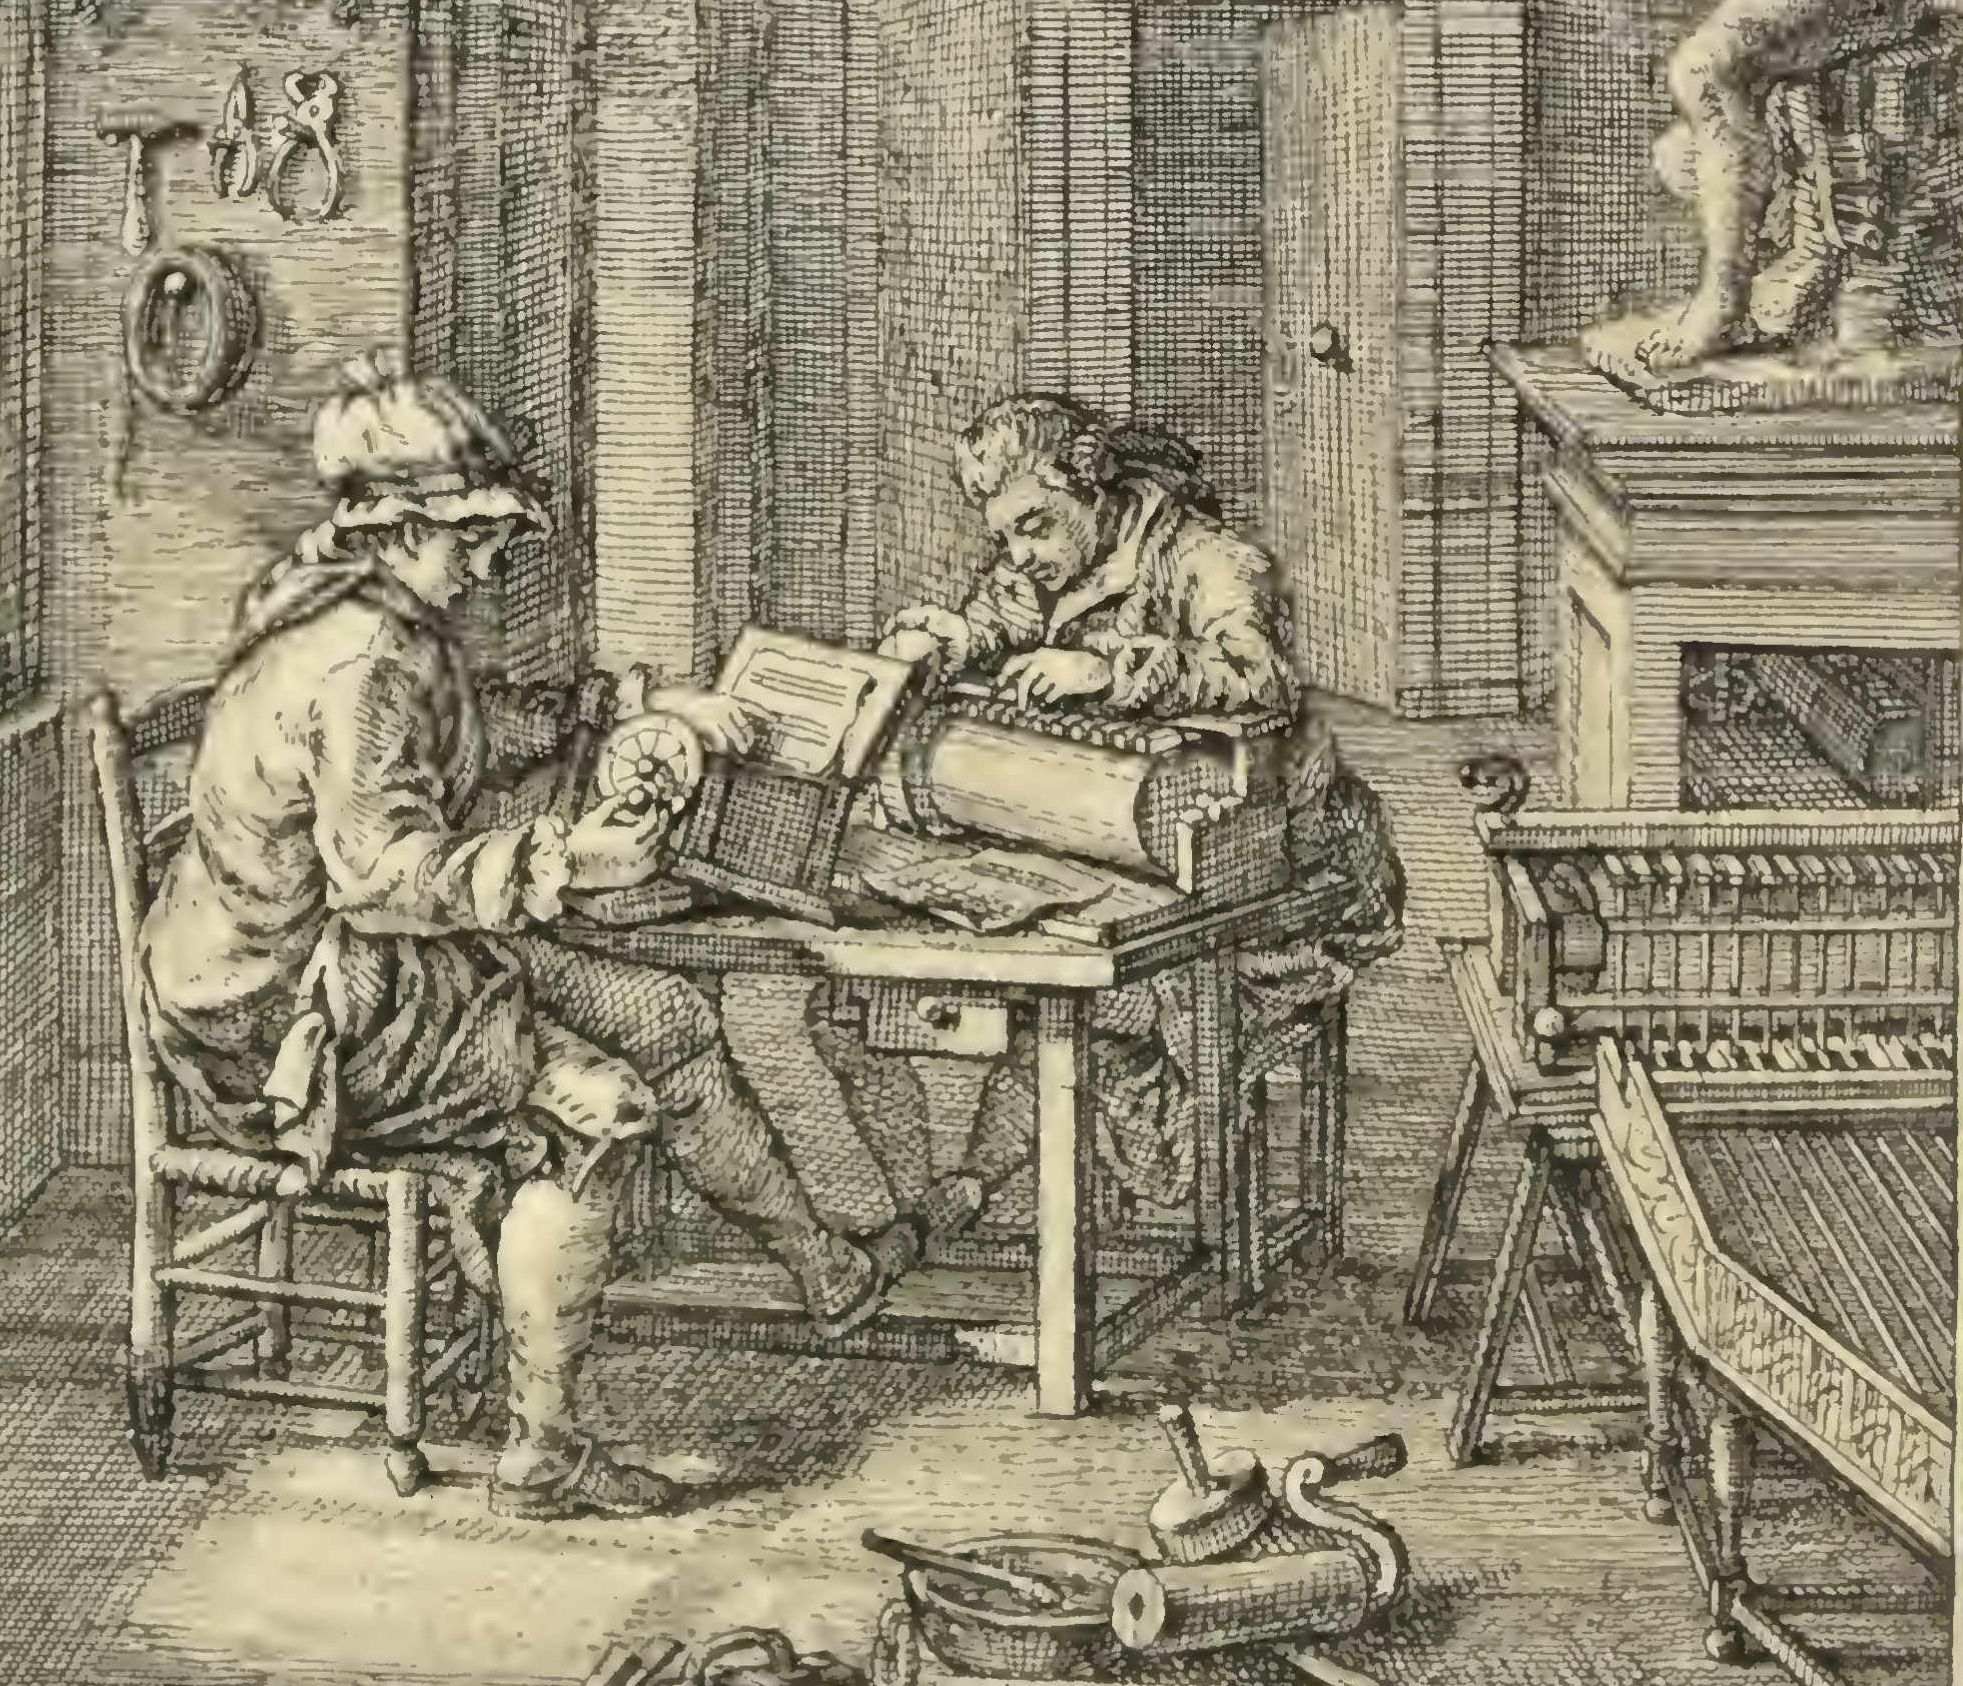
\includegraphics[width=0.9\columnwidth]{./figs/engramelle.jpg}}}
	\caption{Detail from the opening engraved page of Marie-Dominique-Joseph Engramelle \textit{La Tonotechnie ou l’art de noter les cylindres} (1775).} 
	\label{fig:engramelle}
\end{figure}

We can even reassess Henry Purcell’s famous “Wonderous Machine” bass aria from \textit{Ode for St Cecilia’s Day} Z. 328, reinterpreting the lyrics through the lens of an impotent Baroque musician (in this case a lute player) confronting themselves with the infinite possibilities of indefatigable mechanical devices:


\begin{quote}
\begin{center}
\textit{Wondrous machine! \\
To thee the warbling lute, \\
though used to conquest, \\
must be forced to yield, \\
with thee unable to dispute.}
\end{center}
\end{quote}

The voice and instrumental accompaniment's patters seem to emulate the \textit{perpetuum mobile} of mechanically driven musical instruments, the like of which are described in later treatises like Engramelle’s \textit{La Tonotechnie ou l’art de noter les cylindres} (1775) or ambitious implementations such as Diederich Nickolaus Winkel \textit{Componium} (1821), a mechanical device able to play an almost endless amount of variations on a pre-programmed piece of music.\cite{riley2009composing}

\begin{figure}
 \centerline{\framebox{
	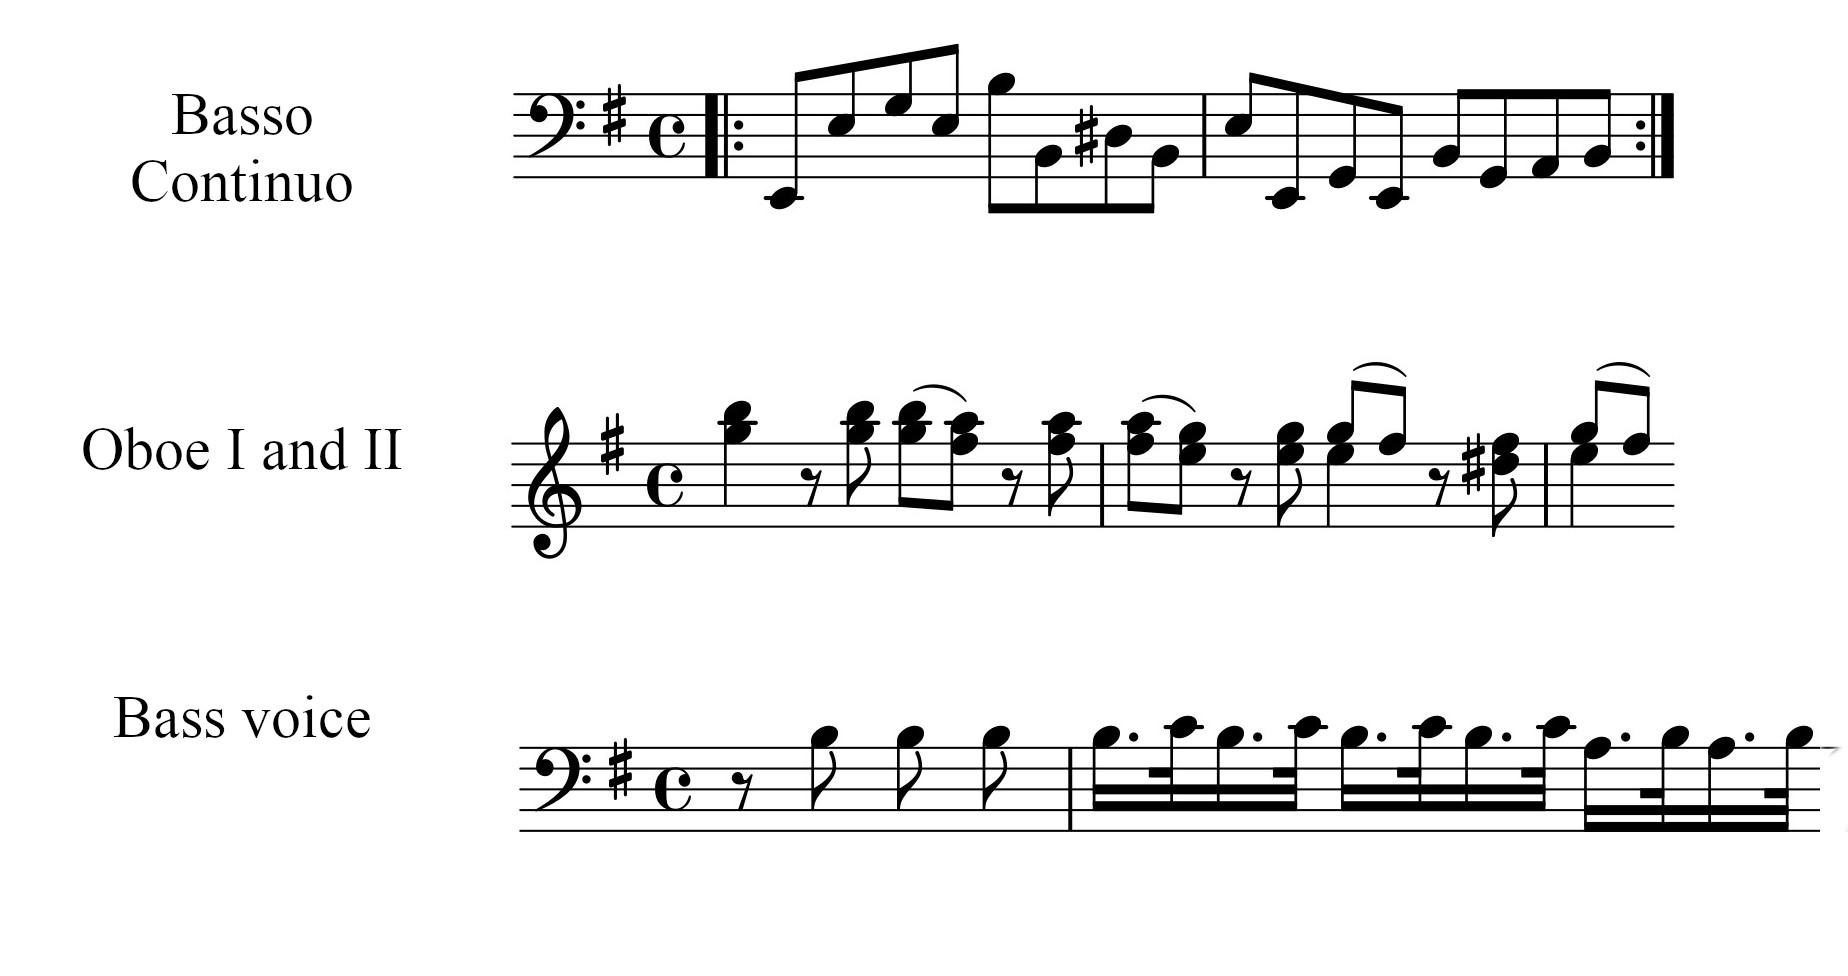
\includegraphics[width=0.9\columnwidth]{./figs/purcell.jpg}}}
	\caption{Opening ground bass, accompaniment of the two oboes and singing voice dotted diminutions of 	respectively measures 1-2, 3-4 and 15-16.}
	\label{fig:purcell}
\end{figure}

But how to translate a highly complex activity, such as music, into an algorithmic procedure? The act of music-making, either planned by a composer or made \textit{ex tempore} by an improviser, arises from selecting musical gestures from an associative knowledge base stored in the musician’s long-term memory.\cite{pressing1998psychological} For centuries, musicians have built such repositories, organising the vast palette of musical gestures, or schemata, through various systems of classification. \cite{berger2005medieval} Tables, decision trees and voice-leading matrices have helped musicians to create a repertoire of melodic, harmonic and rhythmic patterns reflecting their contemporary musical style and performance practice.

%\begin{figure}
 %\centerline{\framebox{
	%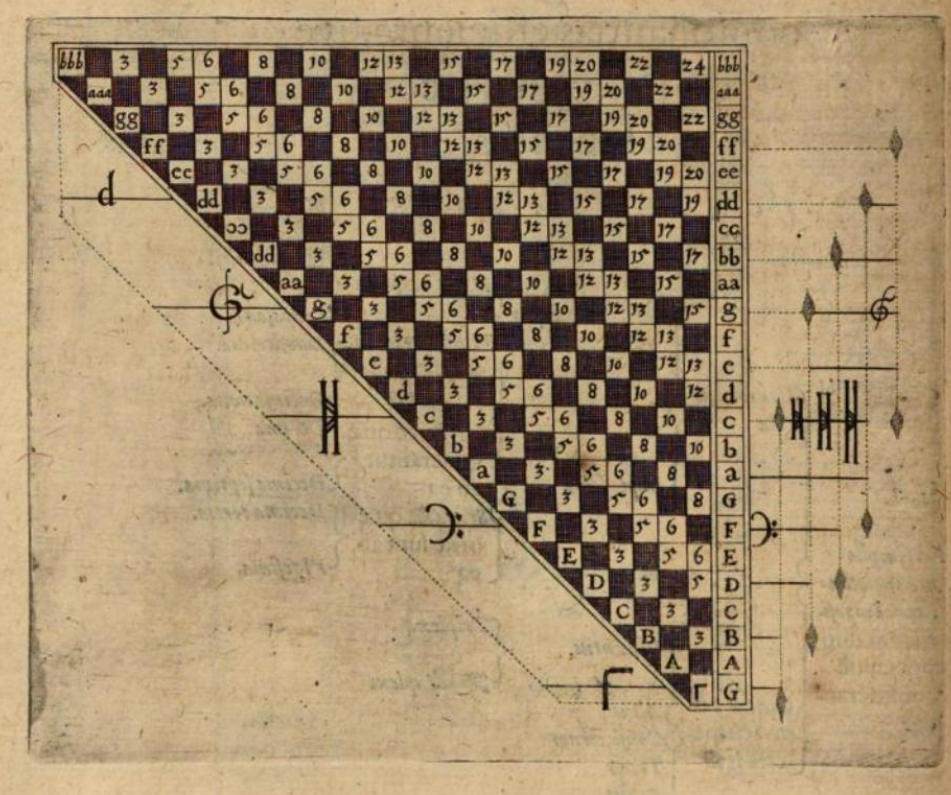
\includegraphics[width=0.9\columnwidth]{./figs/Fludd-De natura simia-II-210.jpg}}}
	%\caption{Table of musical consonances from Robert Fludd \textit{Naturae Simia} (1618), book 2, page 210.}
	%\label{fig:fludd}
%\end{figure}


Archetypical musical schemata were represented by rules, such as Thomas Campion’s procedure for four-voice harmonisation of a given bass line.\cite[p. 1-8]{Campion1618} Moreover, Pietro Cerone encyclopaedic work \textit{El melopeo y maestro},\cite{hannasCeronePhilosopherTeacher1935} provided an endless series of musical tables and examples, similar in fashion to our modern “training sets” for AI models, that musicians internalised in their long term-memory, ready to be used during improvisation or composition of new pieces.\cite{schubertCounterpointPedagogyRenaissance2002}

\begin{figure}
 \centerline{\framebox{
	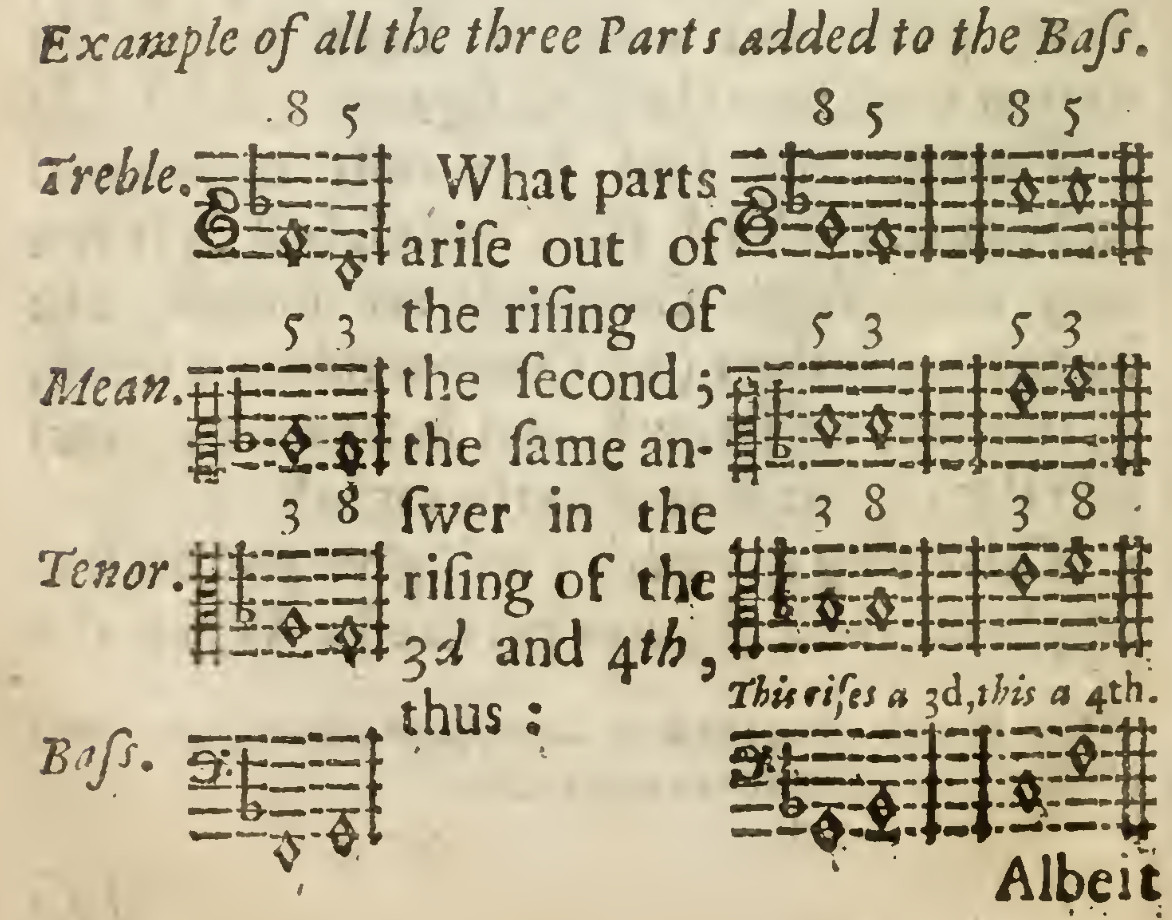
\includegraphics[width=0.9\columnwidth]{./figs/campion.jpg}}}
	\caption{Voice-leadning rules four four-voice harmonisation of a given bass melody. The procedure is based on the bass movements and relative consonances between the upper and lower voices.}
	\label{fig:campion}
\end{figure}

Several treatises, like Giovanni Battista Chiodino’s \textit{Arte Pratica Latina et Volgare di far contrapunto a mente, et a penna} (1610), focussed on contrapuntal patterns that could be used by musicians to harmonise a given melody or bassline, while others, like Francesco Rognoni \textit{Selva de varii passaggi} (1620), provided the students with complex rhythmic patterns for ornamenting melodic lines and cadential formulas not very dissimilar to 20th-century collections like Nicolas Slominsky’s \textit{Thesaurus of Scales and Melodic Patterns} (1947) or Jerry Coker’s \textit{Patterns for Jazz} (1970). 

Of particular interest for our discussion is the ‘Arca Musarithmica’, a computational device designed by the German polymath Athanasius Kircher (1602–1680) and described in the second volume of his \textit{Musurgia Universalis} (1650).\cite{mckay2015musical} Kircher’s compositional tool generates four-voice homophonic and polyphonic harmonisations (respectively named \textit{contrapunctus simplex} and \textit{floridus}) on the basis of a given set of verses and a musical scale, according to the conteporary Renaissance theory of authentic and plagal modes. The machine was designed to generate hymns for Jesuit missionaries working in religious communities outside Europe: thanks to Kircher algorithm, the priests could easily generate music from a liturgical text in the native language of their communities and compose the music according to the “affect” of the verses.\cite{chierotti1994comporre} As if anticipating Purcell’s “Wonderous Machine,” the author describes the algorithm as “wondrous music” (\textit{musurgiae mirificae}), referring to the device’s capacity to instill wonder (\textit{meraviglia}) in listeners and composers (or operators) alike. \footnote{A recent digital implementation of the \textit{arca} has been made by Andrew A. Cashner of University of Rochester. The code is publically available on GitHub at https://github.com/andrewacashner/kircher while a web-based application can be found at https://arca1650.info}
To the best of our knowledge, Kircher is one of the first to use an abstract representation of the four-voice counterpoint: he assigned numerals to the scale's relative degrees and provided tables of rythmical patterns that could be independently assembled with each other. A more "serialistic" approach can be found in the Anonymous treatise \textit{Ludus Melothedicus} (1758), where the author created a series of numerical tables, where each number corresponded to a chromatic pitch and a given duration.
    
%\begin{figure}
 %\centerline{\framebox{
%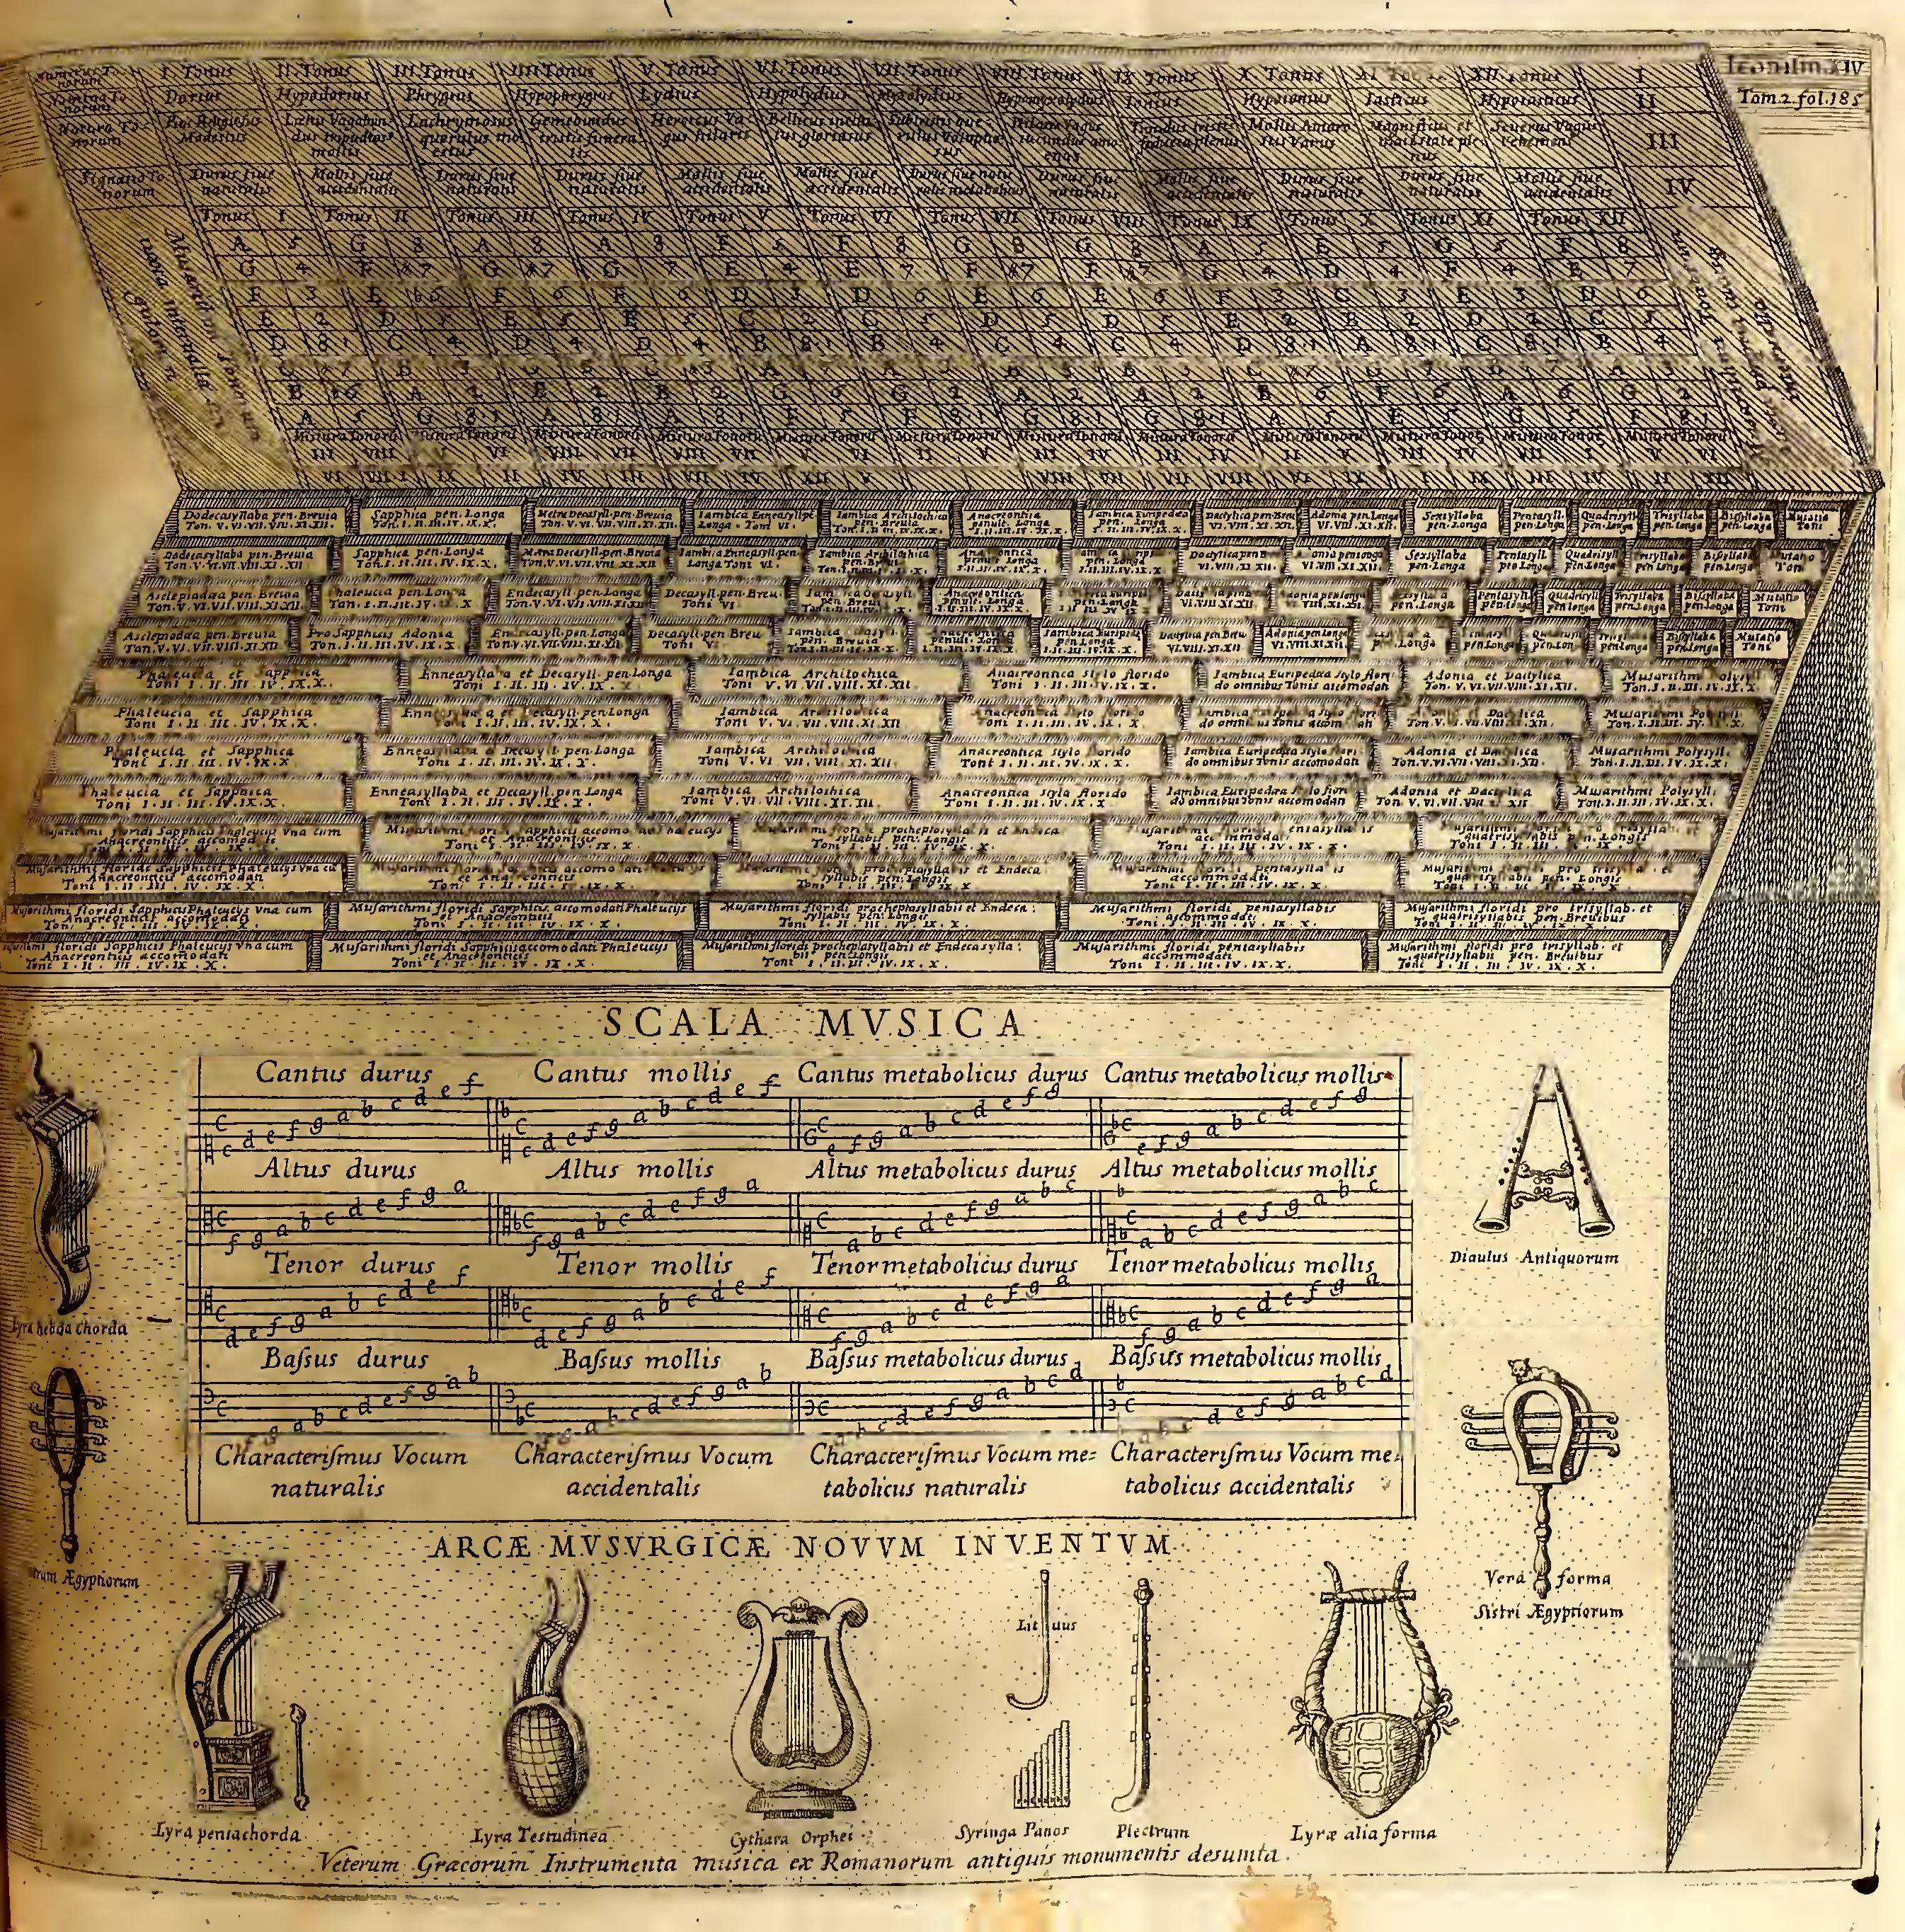
\includegraphics[width=0.9\columnwidth]{./figs/arca.jpg}}}
	%\caption{An illustration of the "arca" from Kircher's original publication, Book 2, page. 185}
	
	%\label{fig:arca}
%\end{figure}

A detailed analysis of Kircher's voice-leading patterns reveals that these four-voice harmonies conform to typical 16th century musical schemata and chord progressions. Many of these progressions are based on counterpoint rules encoded in other treatises, like the one of Thomas Campion, the musical examples of Vicente Lusitano \textit{Introduttione facilissima, et novissima, \dots} (1553), \cite{canguilhem2011singing} Thomas Morley \textit{A Plain and Easy Introduction to Practical Music} (1597) \cite{grimshaw2006morley} and Tomás de Santa María \textit{Libro llamado arte de tañer fantasía} (1565) \cite{roig1994modal}. \cite{wegman2014improvising} 

Furthermore, the idea of encoding contrapuntal structures in a series of mathematical operations has found several resonances in the works of C.P.E. Bach \textit{Einfall einen doppelten Contrapunct in der Octave von 6 Tacten zu machen} (1757), \cite{helmSixRandomMeasures1966} the stylistic analysis of “Palestrina style” counterpoint of Serge Taneiev \textit{Convertible Counterpoint in the Strict Style} (first publication, 1909) \cite{taneievConvertibleCounterpointStrict1962} and in the theories of melody, harmony and rhythmn of 18th century mathematician Leonard Euler.\cite{pesic2013euler}

A step ahead of pure deterministic rules, was the introduction of randomness in the compositional process, reducing the musician's agency on the generated artifact. The development of combinatorics, with its first application to music theory can be found in the early 17th century works of Kircher and Marin Mersenne, musicians explored the possibility of generating music from a series of exemplars through a randomized process, usually implemented by appending musical fragments according to numerical tables and dice rolling. To the best of our knowledge, the first published “dice game” (\textit{würfelspiel} in German) is Johann Philipp Kirnberger \textit{Der allezeit fertige polonoisen- und menüettencomponist} (1757), providing random tables to generate popular dance music (a polonaise and a menuet) for two violins and harpsichord accompaniment. \cite{hedgesDiceMusicEighteenth1978} 

\begin{figure}
 \centerline{\framebox{
	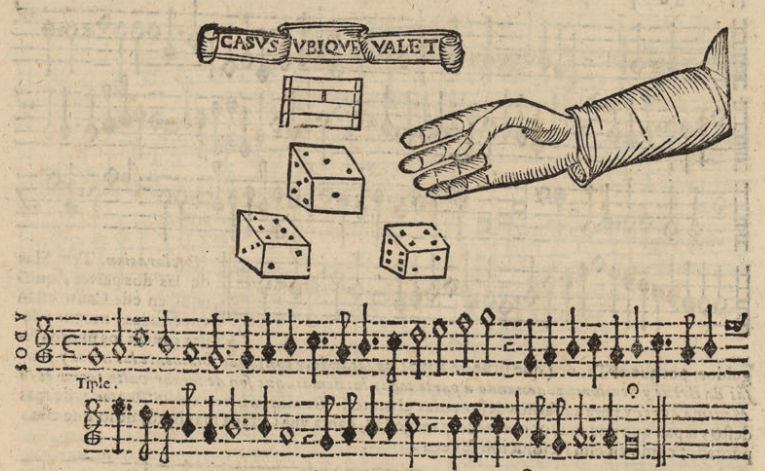
\includegraphics[width=0.9\columnwidth]{./figs/cerone-detail-1124.jpg}}}
	\caption{An erlier example of the use of dice and randomness in musical composition is Pietro Cerone \textit{Enigma de la suerte, ò de los dados} appearing his his \textit{El melopeo y maestro} (1613), pag. 1124. \cite{schiltzCasusUbiqueValet2007}}
	\label{fig:cerone}
\end{figure}

In the coming decades, many other musicians imitated Kirnberger's curious experiment to generate music in an algorithmic fashion, leaving the user’s agency to pure chance. The best known of these "dice games" is probably \textit{Anleitung so viel Walzer oder Schleifer mit zwei Würfeln zu componiren}, attributed to W.A. Mozart and published by Nikolaus Simrock around 1790. Its fame is so great that a digital implementation of the compositional device had already been developed by David Caplin in 1955. \cite{arizaTwoPioneeringProjects2011,hillerMusicComposedComputers1970}

Of particular interest is Antonio Calegari’s \textit{Gioco Pitagorico Musicale} (1801), which provides a framework for including lyrics to the generated airs and duets. In the title the author states clearly that the game is designed “for people without any knowledge of music”,\footnote{"Col quale potrà Ognuno, anco senza sapere di Musica, formarsi una Serie quasi infinita di picciole Ariette"} willing to amuse themselves at home with a seamless infinite combination of songs in the then current operatic style. \cite{bortolozzo1997gioco}

\begin{figure}
 \centerline{\framebox{
	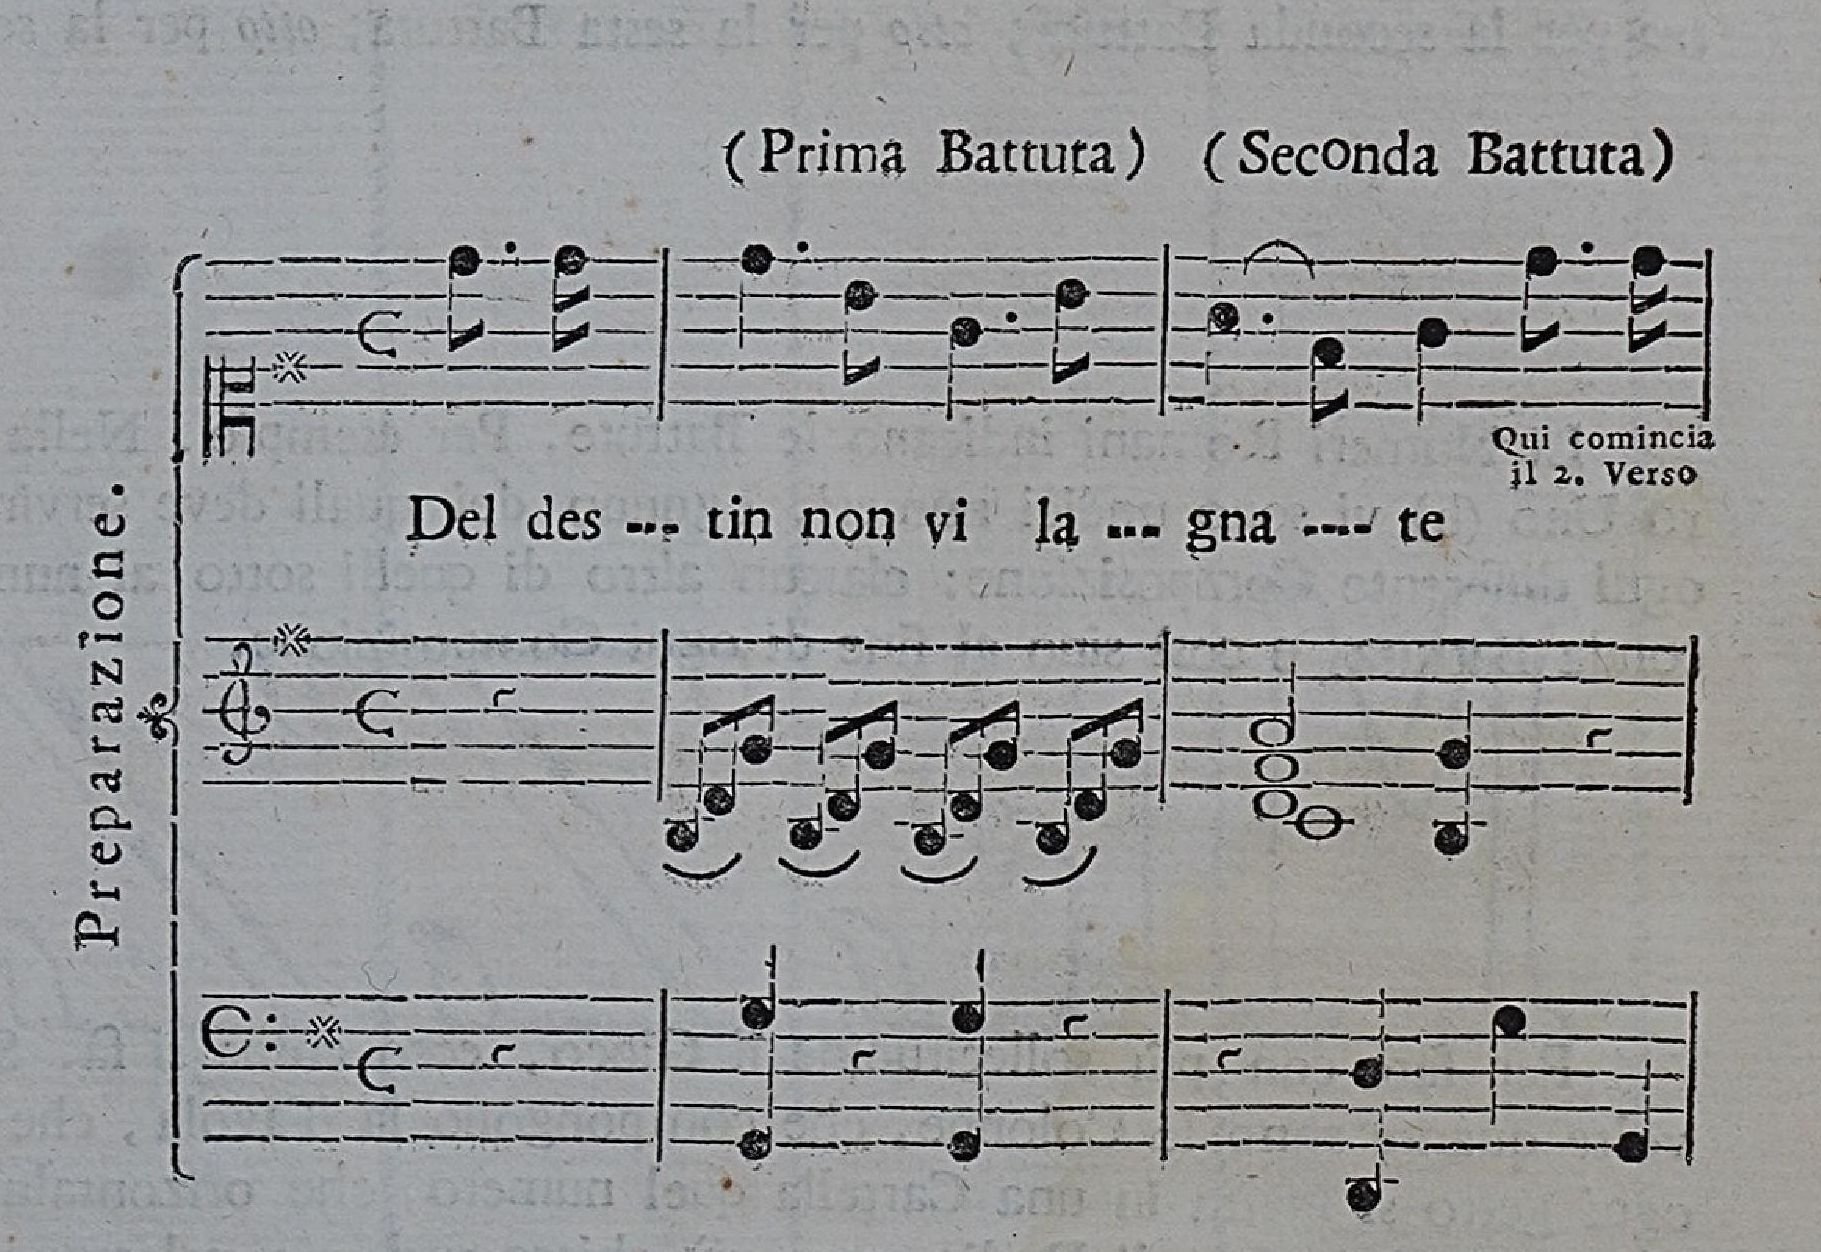
\includegraphics[width=0.9\columnwidth]{./figs/calegari-lyrics.jpg}}}
	\caption{Ingestion of lyrics into the generated music in Calegari's \textit{Gioco Pitagorico Musicale}.}
	
	\label{fig:calegari}
\end{figure}

A similar statement, made in the introduction of Andrea Mangeruva’s \textit{Nuovo Metodo per Comporre Migliaja di Walser} (1839), where the author designed a complicated randomised procedure based on modular arithmetic, encourages the use of the book for domestic music-making and amusement but warns the reader about the “seriousness” of his device: according to Mangeruva a “mechanical musician” (\textit{un musico meccanico}) cannot aspire to “true music” (\textit{la vera musica}), making an analogy between rules and procedures of prosody with the art of poetry. \cite[p. 4]{mangeruvaNuovoMetodoComporre1839}
Unfortunately, Mangeruva's treatise is nothing more than a plagiarism of a 1811 French publication \textit{Barême musical, ou l'Art de composer la musique sans en connaître les principes} attributed to Italian composer Gioseffo Catrufo.  \cite{hedgesDiceMusicEighteenth1978}

\begin{figure}
 \centerline{\framebox{
	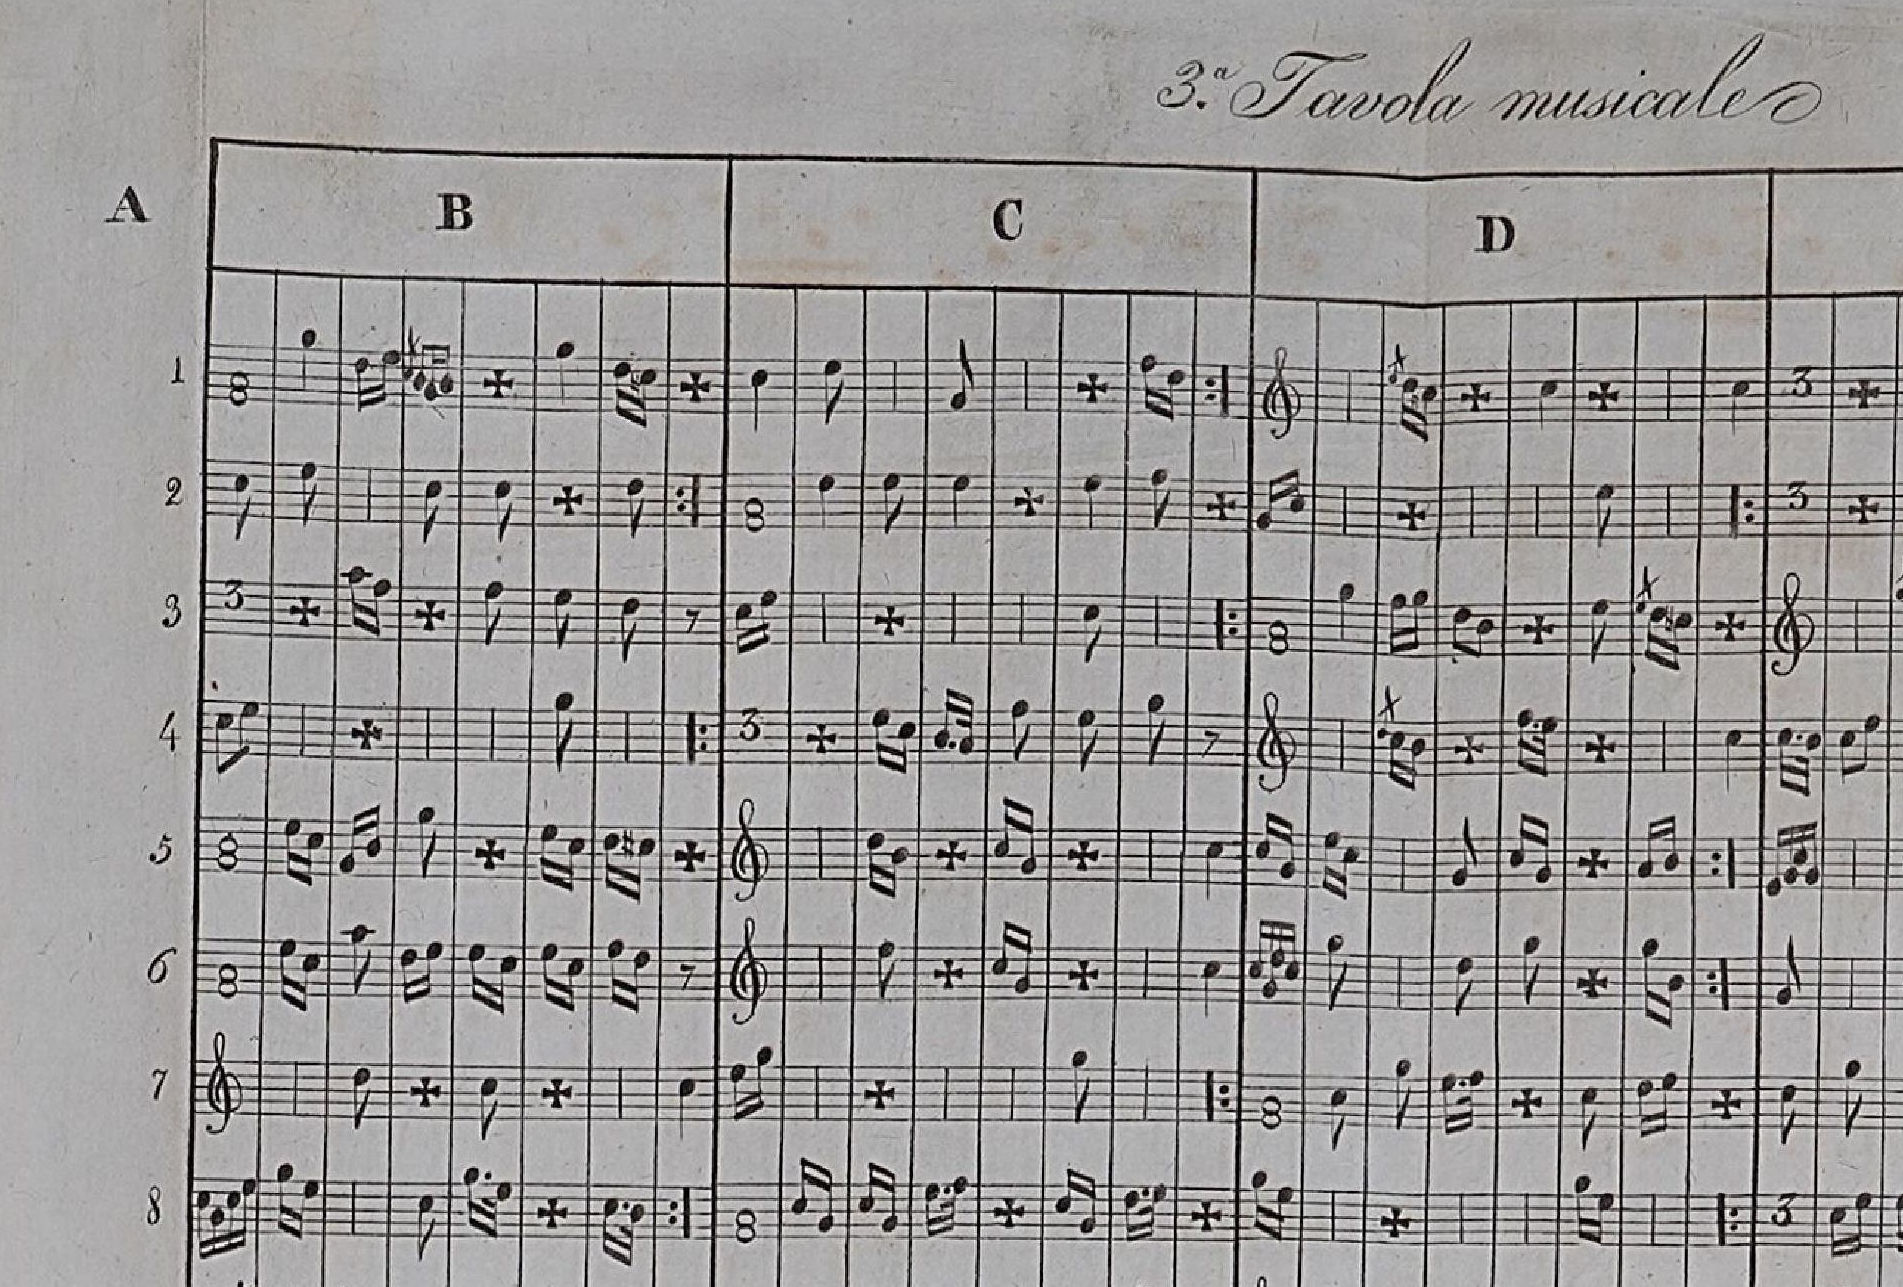
\includegraphics[width=0.9\columnwidth]{./figs/mangeruva-music.jpg}}}
	\caption{Musical table from Andrea Mangeruva \textit{Nuovo Metodo}.}
	
	\label{fig:mangeruva}
\end{figure}

Many of these publications address a specific facet of music-making, namely amusement and entertainment. Is not by chance that these "dice games" were mainly used to generate popular music, in the form of songs and dances. Furthermore, we have noticed how many publishers have attributed their publications to famous composers, such in the case of the \textit{Gioco Filharmonico}, attributed to Joseph Haydn by Luigi Marescalchi in 1793. Misattributions, re-arrangement and even unauthorized reprints have been surprisingly commond in the genre, as previously stated in the instance of Mangeruva's "borrowing" from \textit{Barême musical}.

Concerning the algorithms, they are mostly based on a series of basic musical variations of a piece, like a menuet or countrydance, composed beforehand by the author. Afterwards, a series of puzzles, enigmas, and randomizations are used as expedients to deceive the user, keeping the illusion that the procedure must be of some kind of magic. In several manuscript sources of early "dice games"  the term \textit{cabala} is often used,\footnote{Several 18th century musical dice games refer explicitly to the Jewish kabbalah in their title and content, such as Johann P. Kirnberger \textit{Cabala per componendi minuetti}, Bernardo Ottani \textit{Tavola per la Cabala} and the anonymous \textit{Musicalische Cabala} preserved in the National Library of France. For a detailed list of tretise visit our GitHub repository.}   alluding to the duality between modern science, in the nascent theory of probability, and proto-scientific disciplines like alchemy and astrology. \cite{forshaw2010oratorium} 



\section{Digital implementations}

A series of digital implementations of the treatises described in our paper are publically available on our GitHub repository.\footnote{https://github.com/NicholasCorniaOrpheus/Artyfyshall-Bird} 
Alongside the Python code, we are providing the digital images of the discussed treatises and a small dataset of musical examples in LilyPond\footnote{https://lilypond.org/}, MIDI and PDF format, both from the generated music as for the input exemplars. The transcriptions of each musical fragment could be used as ground truth for Optical Music Recognition tasks involving the transcription of individual measures, both for printed as for handwritten music. \cite{calvo-zaragoza_understanding_2020} Furthermore, this unique musical corpus might be used in future research as baselines for evaluating generative models emulating 18th century Western classical music. A detailed list of pre-digital generative models for music can be found on the aforementioned \textit{Artyfyshall Byrd} GitHub.

\section{Conclusions}

The present article wishes to present the current discussion on Artificial Intelligence and music from an historical perspective. The desire to artificially emulate nature is a fascinating feature of human beings, and can find its roots in history, as well as in myths like Pygmalion, described in Ovid's Metamorphoses (c. 8 CE), Book X. \cite[p. 128-148]{ovidmethapores1997} With the technological developments of the Modern Period we have increasingly refined our craft to a point where the differences between the `artificial` and the `natural`, between the `authentic` and the `forged`, are almost impossibile to discern. \cite{battin1979exact}
On the other hand, the challenges afforded by technology and its artificial devices encourage us to reconsider the meaning of creativity and the role of art in our culture. \cite{colton2012computational}
New technologies pose a "challenge to the imagination"  for composers and performers, \cite{lincoln2019computer} extending the boundaries of human's creative effort. This statement is still valuable to our modern "wondrous" times, where the dreams of Leonard Euler \cite{grant2013leonhard} and Ada Lovelace \footnote{Once the fundamental features of sound can be encoded in expressions interpretable by a machine, then "the engine might compose elaborate and scientific pieces of music of any degree of complexity or extent."} \cite{bowles1970musicke} to mathematically encode every facet of music so that a machine could generate new pieces have become a tangible reality. Studing what it meant for our forerunnes to interact with the wonders of \textit{musurgiae mirificae} can help us frame the current issue from a historical, dialectical perspective.

\section{Acknowledgments}

We are particulary grateful to the library staff of the Conservatory of Venice Benedetto Marcello (Paolo da Col and Silvia Urbani) for the digital images of Mangeruva and Calegari treatises. We are also thankful to the Abjad developpers for providing a useful Python library compatible with the Lilypond music encoding syntax \cite{baca2015abjad}.



% For bibtex users:
\bibliography{Orpheus-ISMIR2024}



\end{document}

